\documentclass[10pt]{dokument-ppi}

\begin{document}


\Cwiczenie{Ćwiczenie 3}
\Meta
\Tytul{Harmonogram pracy}
\Data{2012-11-24}
\Autorzy{TC}
\MakeDokumentMeta


\section{Harmonogram pracy}

Znajduje się na stronie \pageref{fig:harmonogram}.

\begin{figure}[p]
    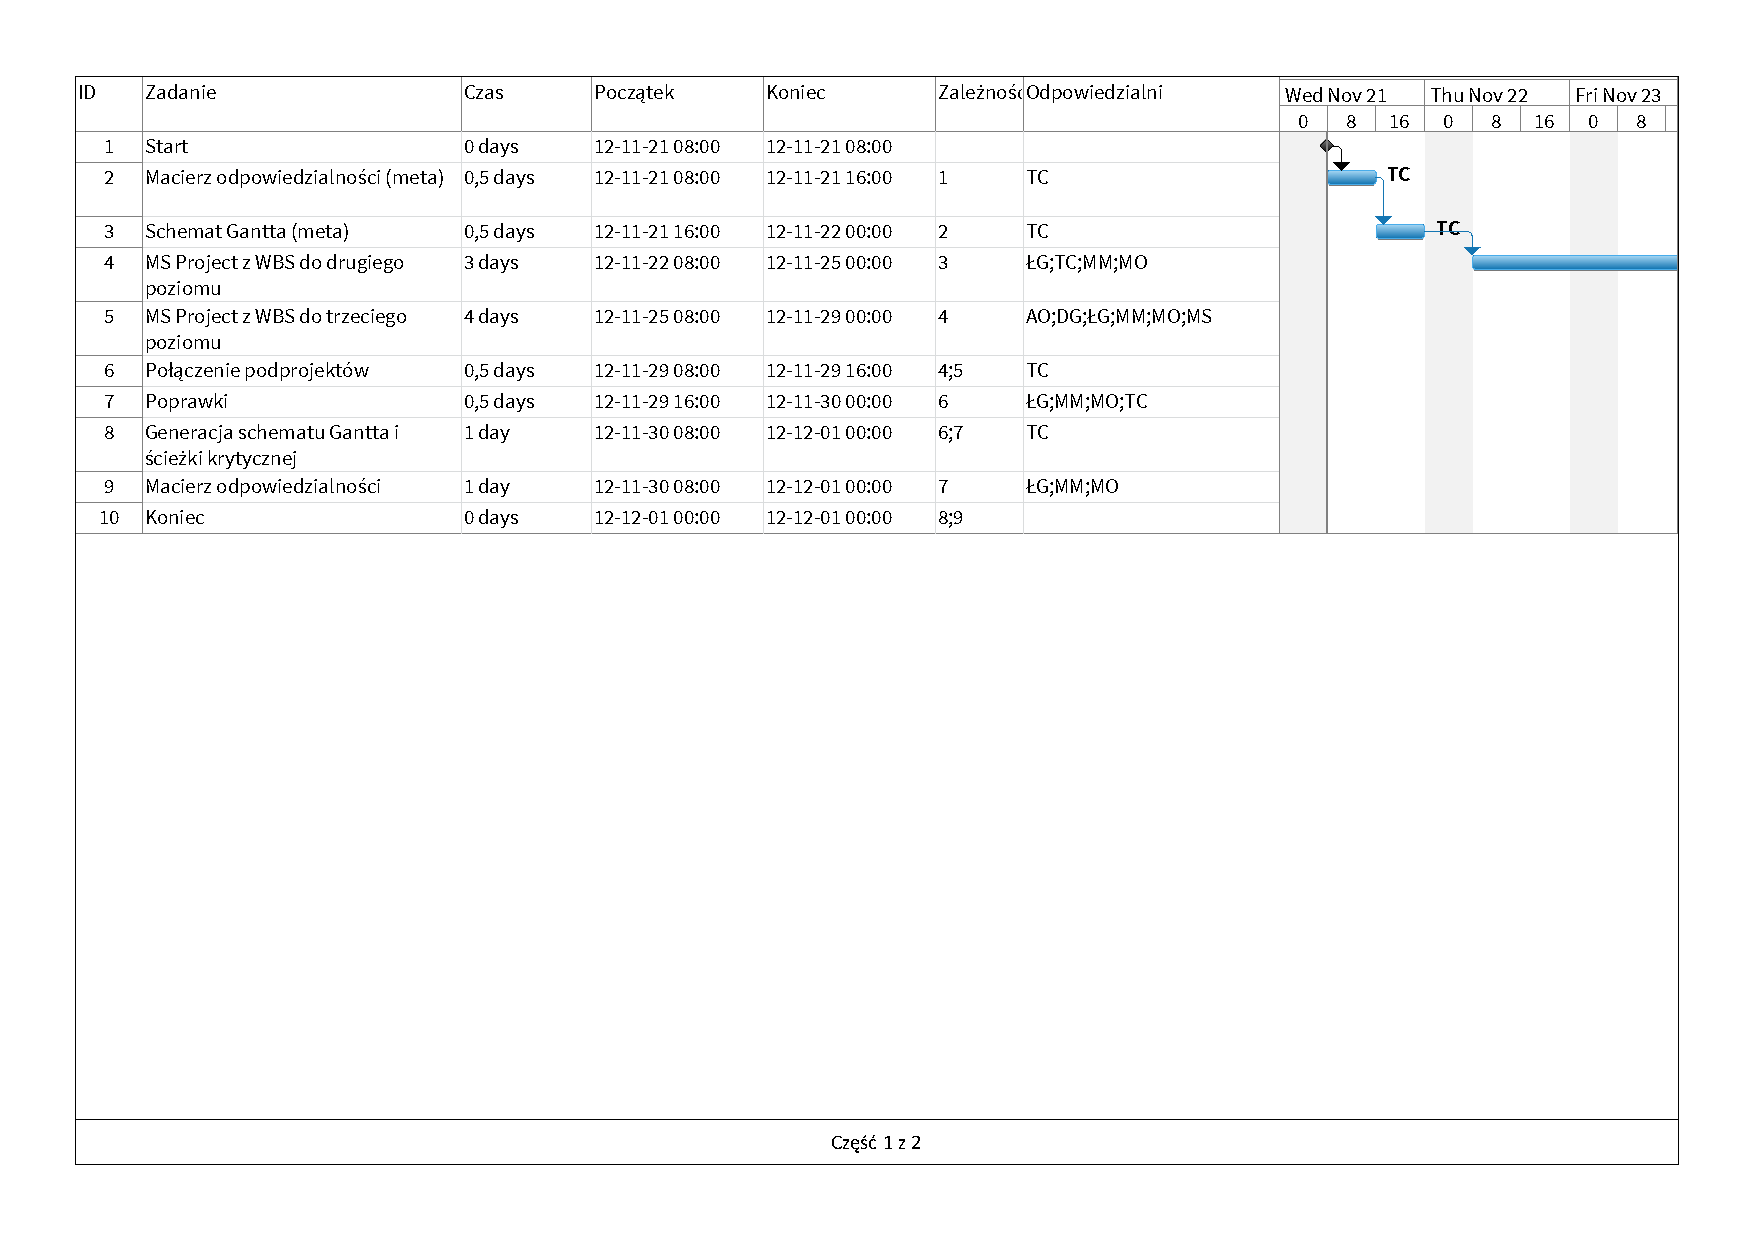
\includegraphics[trim=1.23cm 1.23cm 1.23cm 1.23cm,page=1,angle=270,width=\textwidth]{./figury/harmonogram}
    \caption{Harmonogram pracy w ramach ćwiczenia 3.}
    \label{fig:harmonogram}
\end{figure}

\begin{figure}[p]
    \ContinuedFloat
    \includegraphics[trim=1.23cm 1.23cm 1.23cm 1.23cm,page=2,angle=270,width=\textwidth]{./figury/harmonogram}
    \caption[]{Harmonogram pracy w ramach ćwiczenia 3. (kontynuacja)}
\end{figure}


\section{Historia dokumentu}
\begin{versions}
    \version*{1.0}{2012-11-24}{TC}%
        Dodano pełen harmonogram pracy.
\end{versions}


\end{document}
